\section{Présentation du cours}

\frame{
    \frametitle{Organisation du cours}

    \begin{block}{Organisation des séances}
        \begin{description}
            \item[CM~:] notions de base sur les graphes, présentation d'algorithmes classiques, exemple de présentation
            \item[TD~:] travail de recherche par groupe sur une application des graphes ou un sujet théorique plus avancé, présentation au reste de la classe
        \end{description}
    \end{block}

    \begin{block}{Évaluation}
        \begin{description}
            \item[50\%] tests sur le cours en début de séances
            \item[50\%] présentation des sujets de TD
        \end{description}
    \end{block}
}

\frame{
    \frametitle{Pourquoi étudier les graphes}

    \begin{block}{Graphe}
        Outil de \enavant{modélisation} permettant de représenter les relations entre les éléments d'un ensemble fini :
        \begin{itemize}
            \item routes et distances entre villes,
            \item liens hypertext entre pages web,
            \item etc
        \end{itemize}
    \end{block}

    \begin{block}{Algoritmes}
        Pour analyser les relations représentées par un graphe :
        \begin{itemize}
            \item trouver le plus court trajet entre deux villes,
            \item étudier les groupes sociaux sur internet,
            \item etc
        \end{itemize}
    \end{block}
}

\frame{
    \frametitle{Exemple d'application~: théorème des 4 couleurs}
    \hspace*{-0.5cm}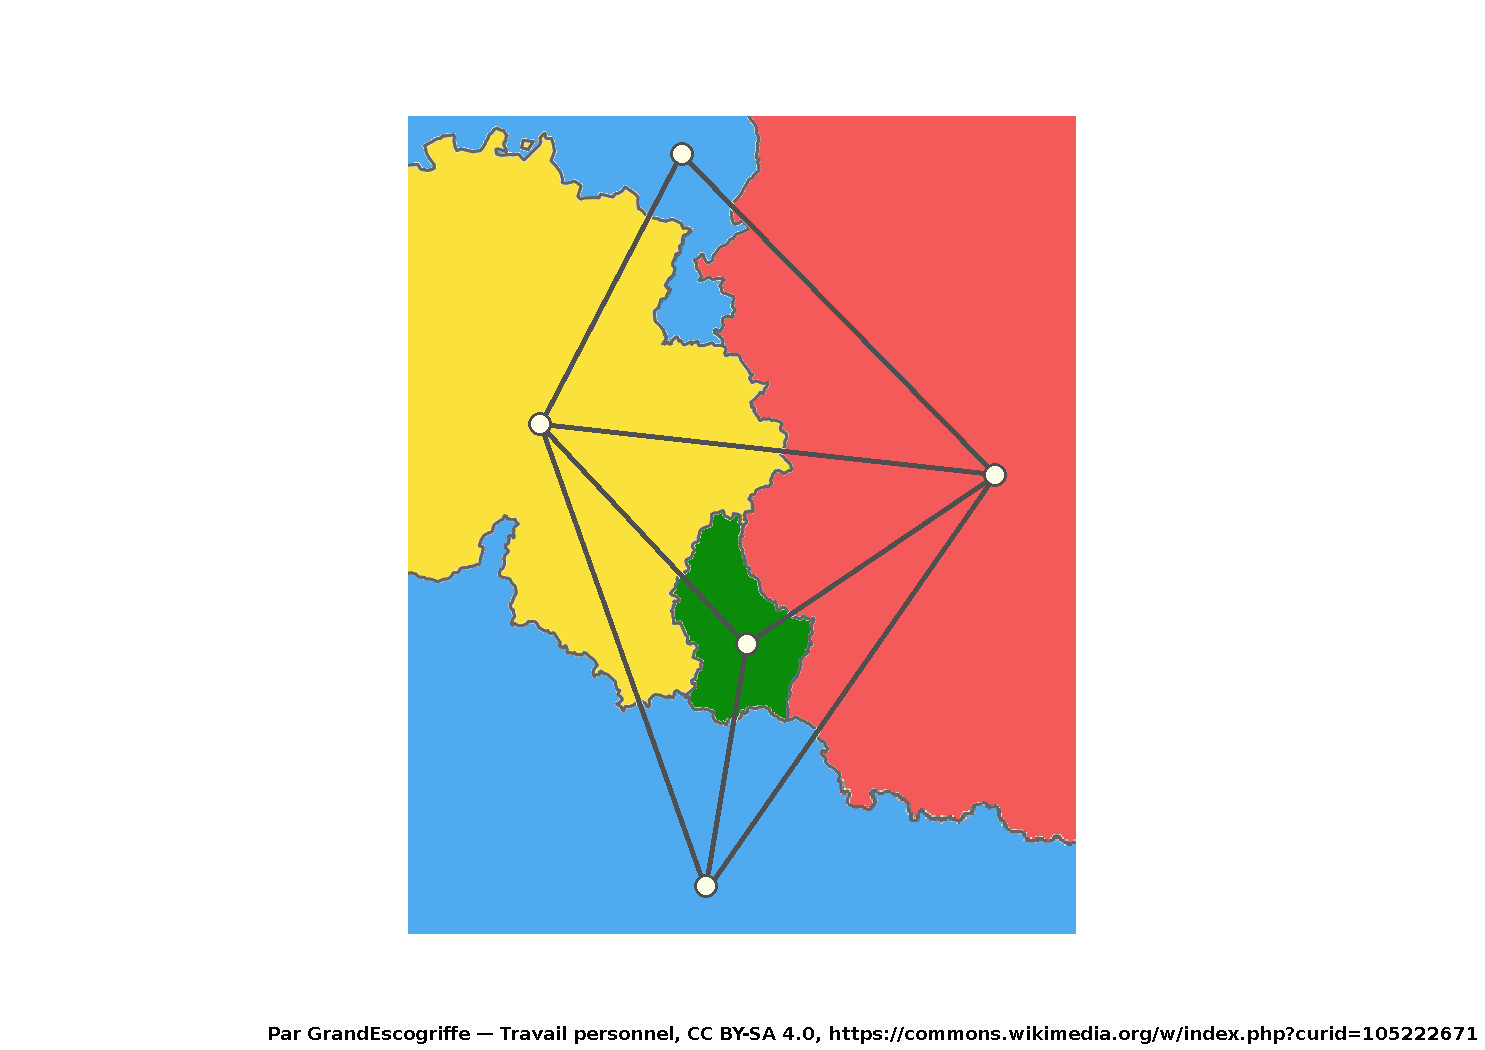
\includegraphics[width=12cm]{1-quatrecouleurs.jpg}
}

\frame{
    \frametitle{Exemple d'application~: sortir d'un labyrinthe}
    \hspace*{-0.5cm}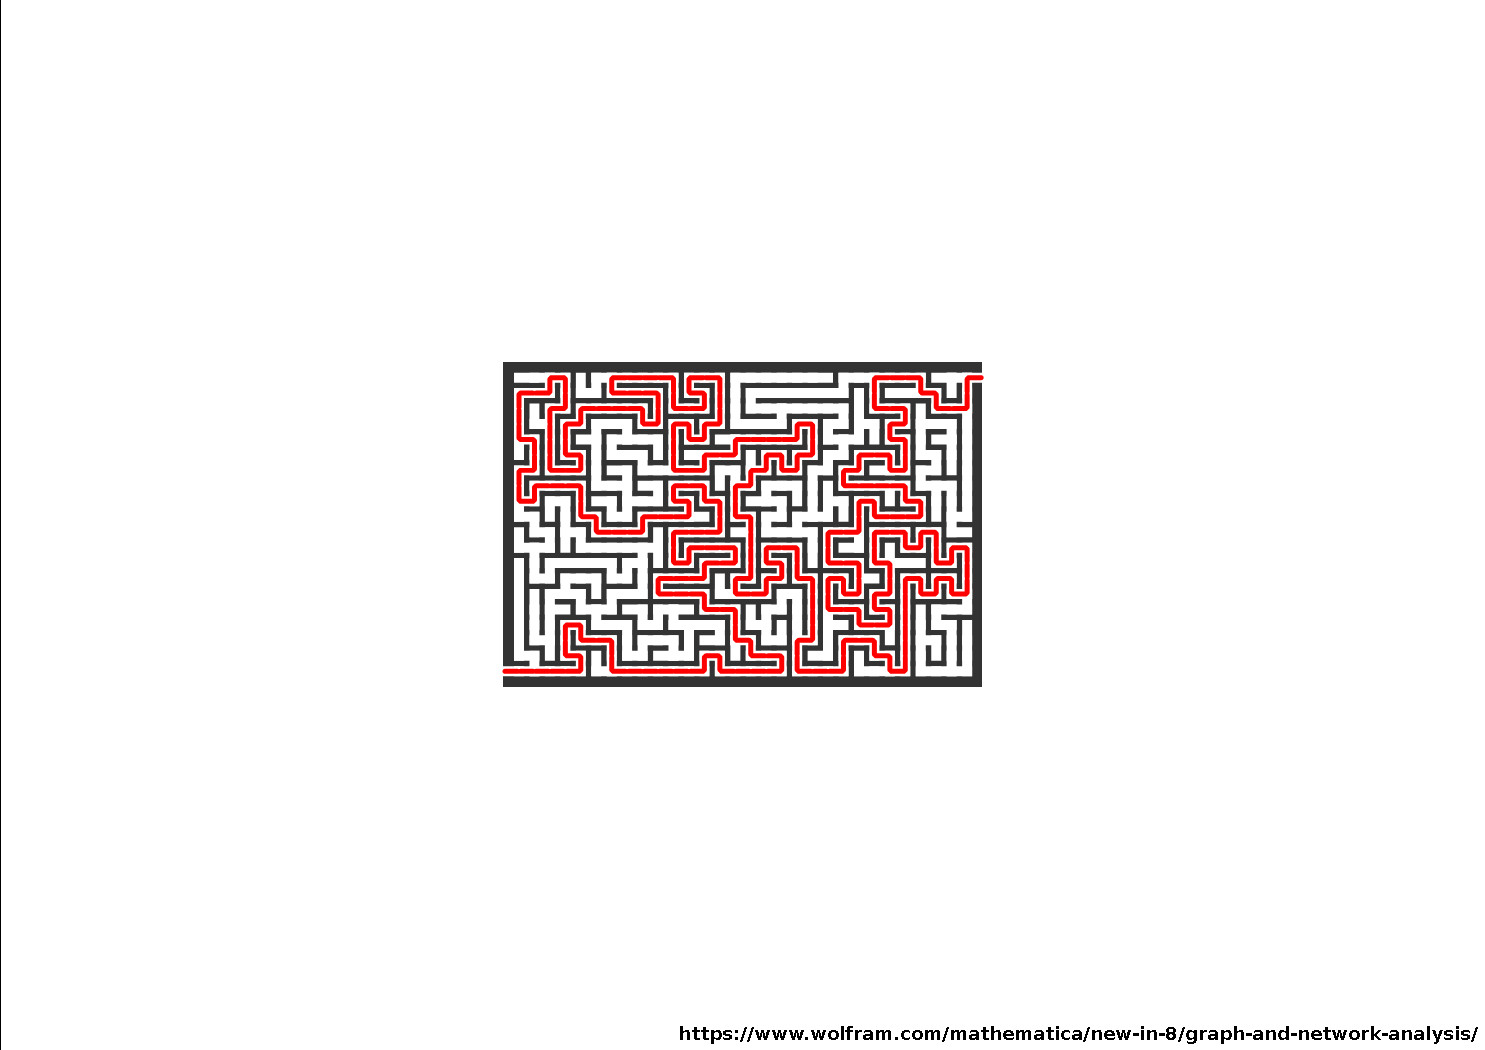
\includegraphics[width=12cm]{2-lab.jpg}
}

\frame{
    \frametitle{Exemple d'application~: recherche d'itinéraire}
    \hspace*{-0.5cm}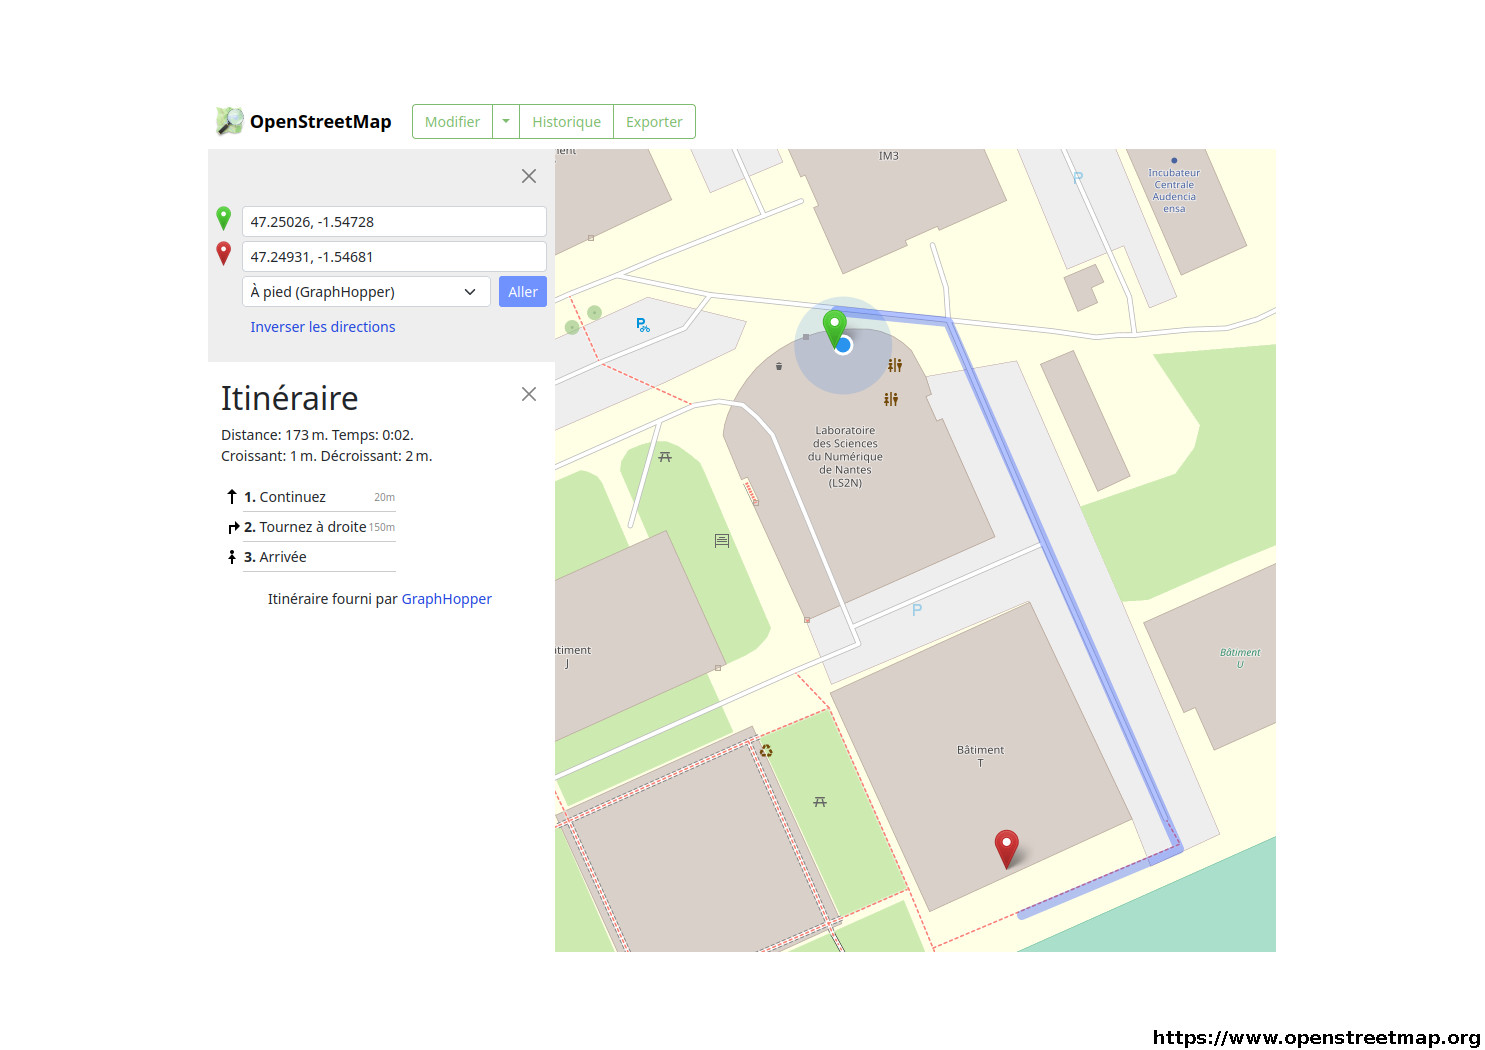
\includegraphics[width=12cm]{3-map.jpg}
}

\frame{
    \frametitle{Exemple d'application~: représentation du web}
    \hspace*{-0.5cm}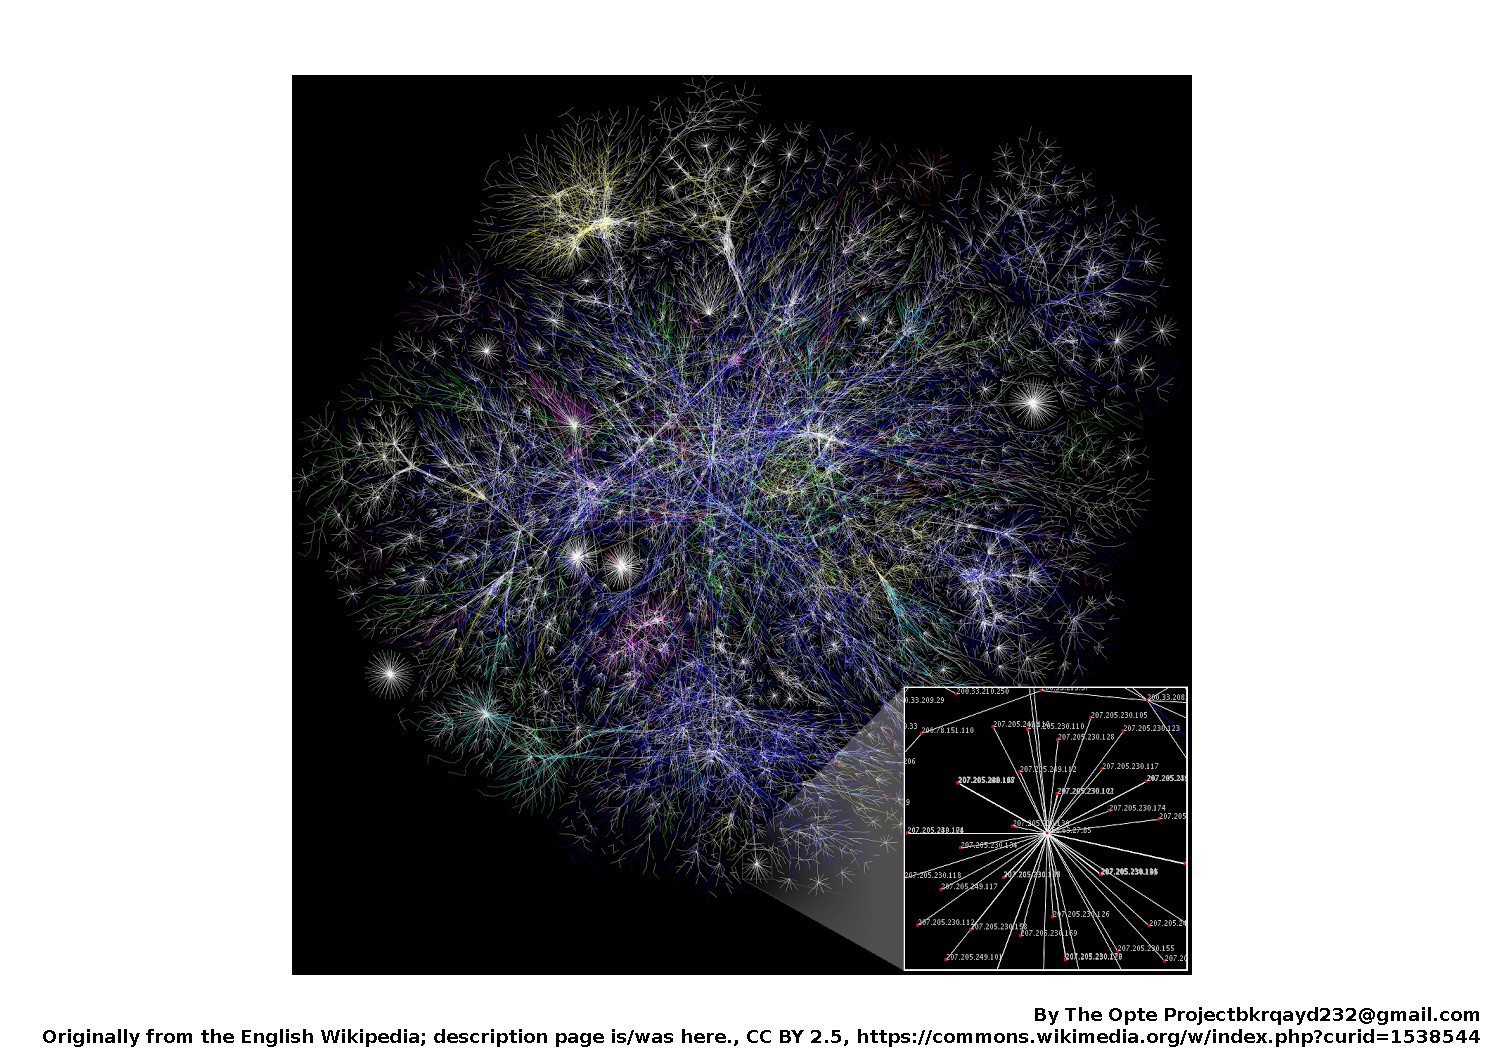
\includegraphics[width=12cm]{4-carteduweb.jpg}
}

\frame{
    \frametitle{Exemple d'application~: réseaux neuronaux}
    \hspace*{-0.5cm}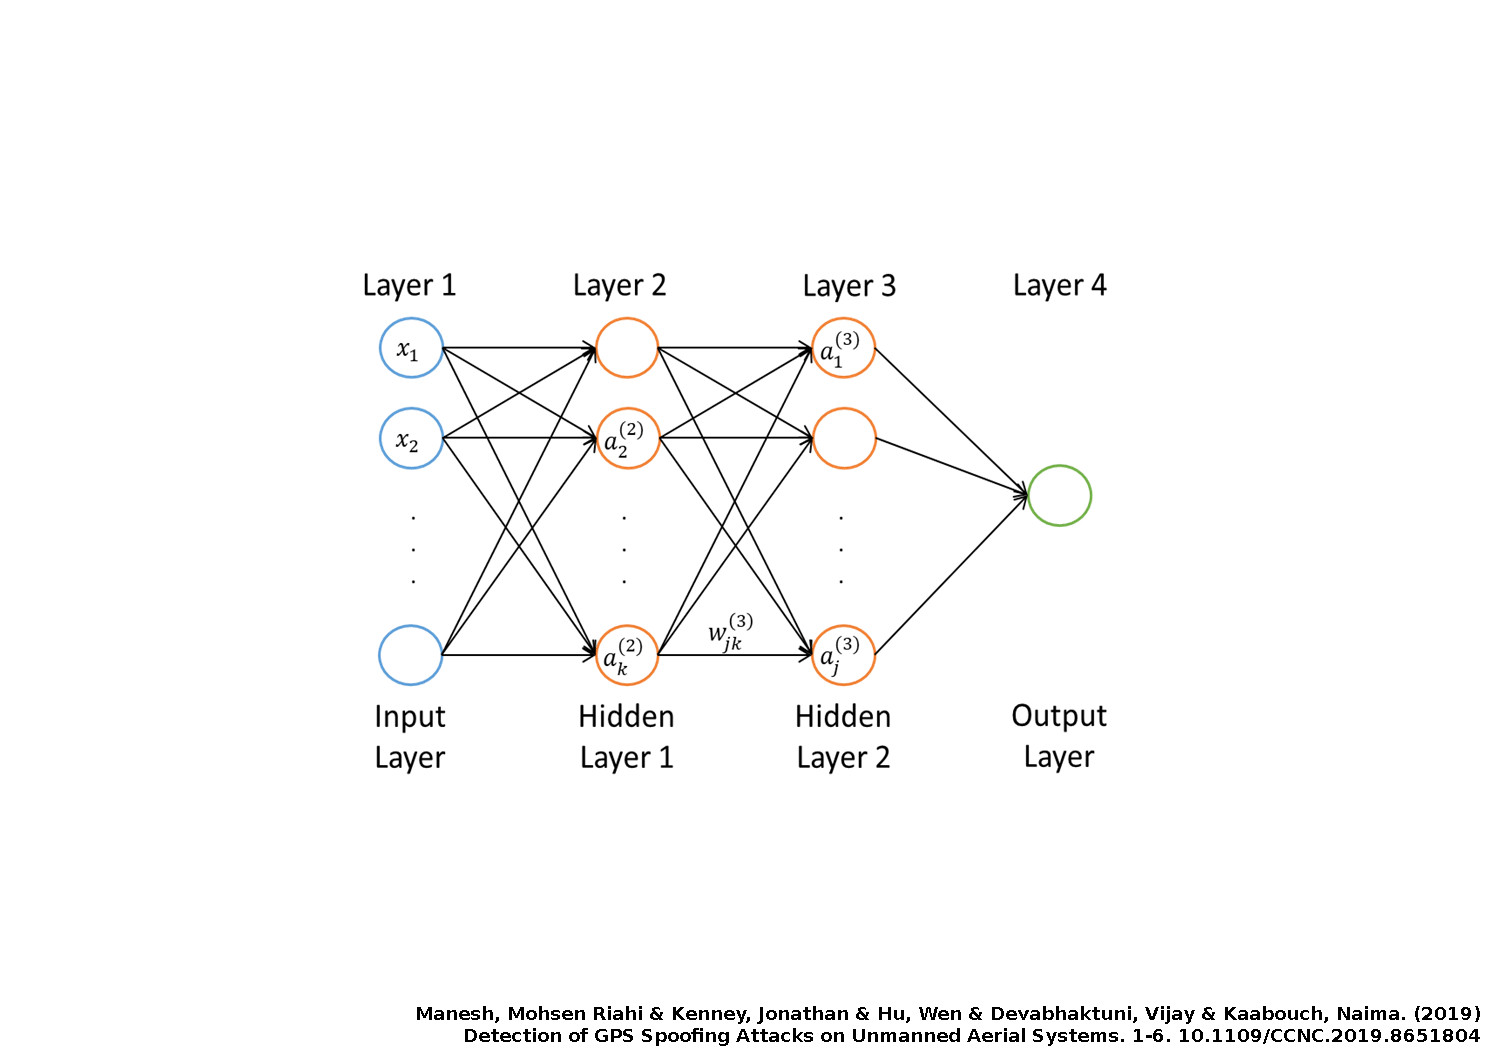
\includegraphics[width=12cm]{5-neuralnetwork.jpg}
}

\frame{
    \frametitle{Sujets de recherche}

    \begin{enumerate}
        \item Représenter graphiquement les grands graphes
        \item Systèmes multi-agents~: exploration collaborative d'un graphe
        \item Recherche de chemins, algorithme A*
        \item Construire la carte d'internet
        \item Marches aléatoires sur les graphes
        \item Graphes planaires et mineurs exclus
        \item Graphes petit-mondes
        \item Réécriture de graphes
        \item Graphes et recommandation "top-N"
        \item Hypergraphes
    \end{enumerate}
}